\documentclass{standalone}
\usepackage{tikz}
\usepackage{pgfplots}

\pgfplotsset{compat = newest}

\definecolor{color_green3}{RGB}{0,150,0}
\definecolor{purple}{RGB}{140,0,190}
\definecolor{blue_green}{RGB}{0,190,190}

\begin{document}
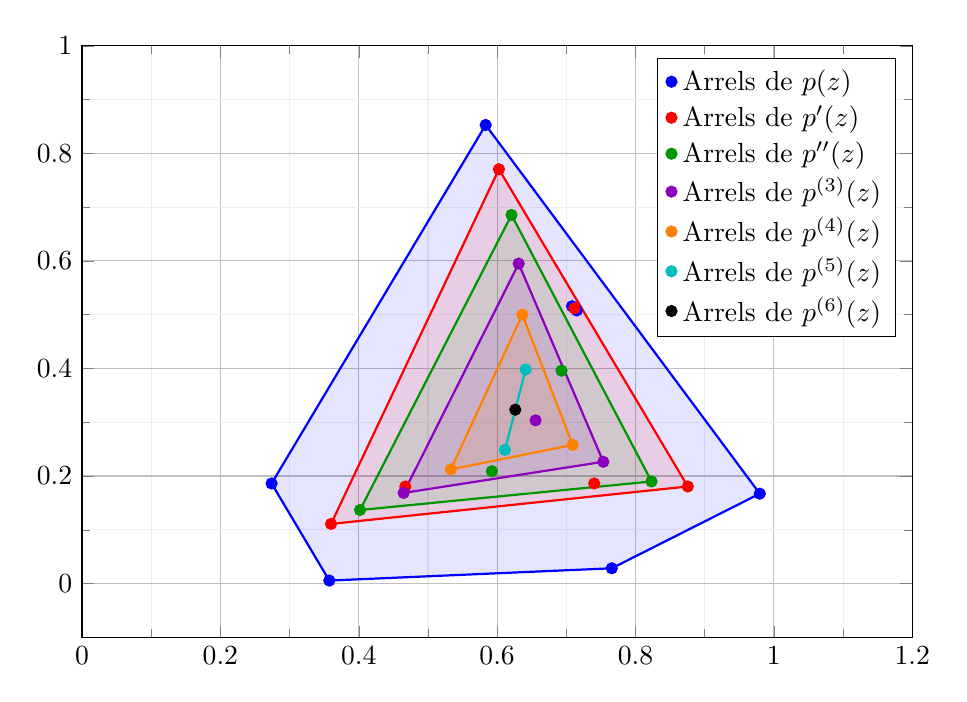
\begin{tikzpicture}
    \begin{axis}[
            xmin = 0, xmax = 1.2, %
            ymin = -0.1, ymax = 1, %
            xtick distance = 0.2, %Is the distance between major ticks in the x-axis.
            ytick distance = 0.2, %Is the distance between major ticks in the y-axis.
            grid = both, %When this options is set to both the minor and major grid are plotted.
            minor tick num = 1, %Is the number of ticks between major ticks.
            major grid style = {lightgray}, %Changes the color and stroke of the major grid.
            minor grid style = {lightgray!25}, %Changes the color and stroke of the minor grid.
            width = \textwidth, %sets the width of the figure
            height = 0.75\textwidth,  %sets the height of the figure
            xlabel = {}, %
            ylabel = {}, %
            legend cell align = {left}, %
            legend style={} % position of the legend box and anchor is the point on the box to be fitted exactly at the point of cs:<>,<>. Options are anchor=center,south west,south east,north west,north east,north,south,west... Example: legend style={at={(axis cs:0,-0.5)},anchor=center}
        ]
        %% K(P), where P=(x - 0.273994495981102 - 0.186176450319403*I)*(x - 0.357383151761803 - 0.00556170295068669*I)*(x - 0.583390911966438 - 0.852776648628168*I)*(x - 0.708283194910822 - 0.515710545020349*I)*(x - 0.715180650502866 - 0.507858210223678*I)*(x - 0.765699868206733 - 0.0284062266659330*I)*(x - 0.979617456644666 - 0.167189780830185*I)
        \draw[blue, thick, fill=blue, fill opacity=0.1] (0.58339, 0.85277) -- (0.97961, 0.16718) -- (0.76569, 0.028406) -- (0.35738, 0.0055617) -- (0.27399, 0.18617) -- cycle;
        %% K(P')
        \draw[red, thick, fill=red, fill opacity=0.1] (0.60255, 0.77049) -- (0.87559, 0.18054) -- (0.35990, 0.11090) -- cycle;
        %% K(P'')
        \draw[color_green3, thick, fill=color_green3, fill opacity=0.1] (0.62076, 0.68548) -- (0.82315, 0.18989) -- (0.40175, 0.13673) -- cycle;
        %% K(P''')
        \draw[purple, thick, fill=purple, fill opacity=0.1] (0.63113, 0.59496) -- (0.46479, 0.16856) -- (0.75344, 0.22645) -- cycle;
        %% K(P'''')
        \draw[orange, thick, fill=orange, fill opacity=0.1] (0.53302, 0.21224) -- (0.63637, 0.50009) -- (0.70925, 0.25780) -- cycle;
        %% K(P''''')
        \draw[blue_green, thick, fill=blue_green, fill opacity=0.1] (0.61126, 0.24862) -- (0.64117, 0.39814);
        %% roots of polynomial the polynomial P
        \addplot[only marks,blue,mark=oplus*,mark size=2pt] coordinates {
                (0.35738, 0.0055617)
                (0.27399, 0.18617)
                (0.76569, 0.028406)
                (0.70828, 0.51571)
                (0.58339, 0.85277)
                (0.97961, 0.16718)
                (0.71518, 0.50785)
            };
        %% roots of 1st derivative of polynomial P
        \addplot[only marks,red,mark=oplus*,mark size=2pt] coordinates {
                (0.35990, 0.11090)
                (0.46730, 0.18048)
                (0.87559, 0.18054)
                (0.74028, 0.18610)
                (0.71167, 0.51176)
                (0.60255, 0.77049)
            };
        %% roots of 2nd derivative of polynomial P
        \addplot[only marks,color_green3,mark=oplus*,mark size=2pt] coordinates {
                (0.40175, 0.13673)
                (0.82315, 0.18989)
                (0.59234, 0.20892)
                (0.69308, 0.39587)
                (0.62076, 0.68548)
            };
        %% roots of 3rd derivative of polynomial P
        \addplot[only marks,purple,mark=oplus*,mark size=2pt] coordinates {
                (0.46479, 0.16856)
                (0.63113, 0.59496)
                (0.65551, 0.30355)
                (0.75344, 0.22645)
            };
        %% roots of 4th derivative of polynomial P
        \addplot[only marks,orange,mark=oplus*,mark size=2pt] coordinates {
                (0.53302, 0.21224)
                (0.63637, 0.50009)
                (0.70925, 0.25780)
            };
        %% roots of 5th derivative of polynomial P
        \addplot[only marks,blue_green,mark=oplus*,mark size=2pt] coordinates {
                (0.61126, 0.24862)
                (0.64117, 0.39814)
            };
        %% roots of 6th derivative of polynomial P
        \addplot[only marks,black,mark=oplus*,mark size=2pt] coordinates {
                (0.62622, 0.32338)
            };
        \legend{Arrels de $p(z)$,Arrels de $p'(z)$,Arrels de $p''(z)$,Arrels de $p^{(3)}(z)$,Arrels de $p^{(4)}(z)$,Arrels de $p^{(5)}(z)$,Arrels de $p^{(6)}(z)$}
    \end{axis}

\end{tikzpicture}
\end{document}